% Figure: Compartmental Energy Model
% Shows 4-compartment energy flow with CNS as bottleneck

\begin{figure}[htbp]
\centering
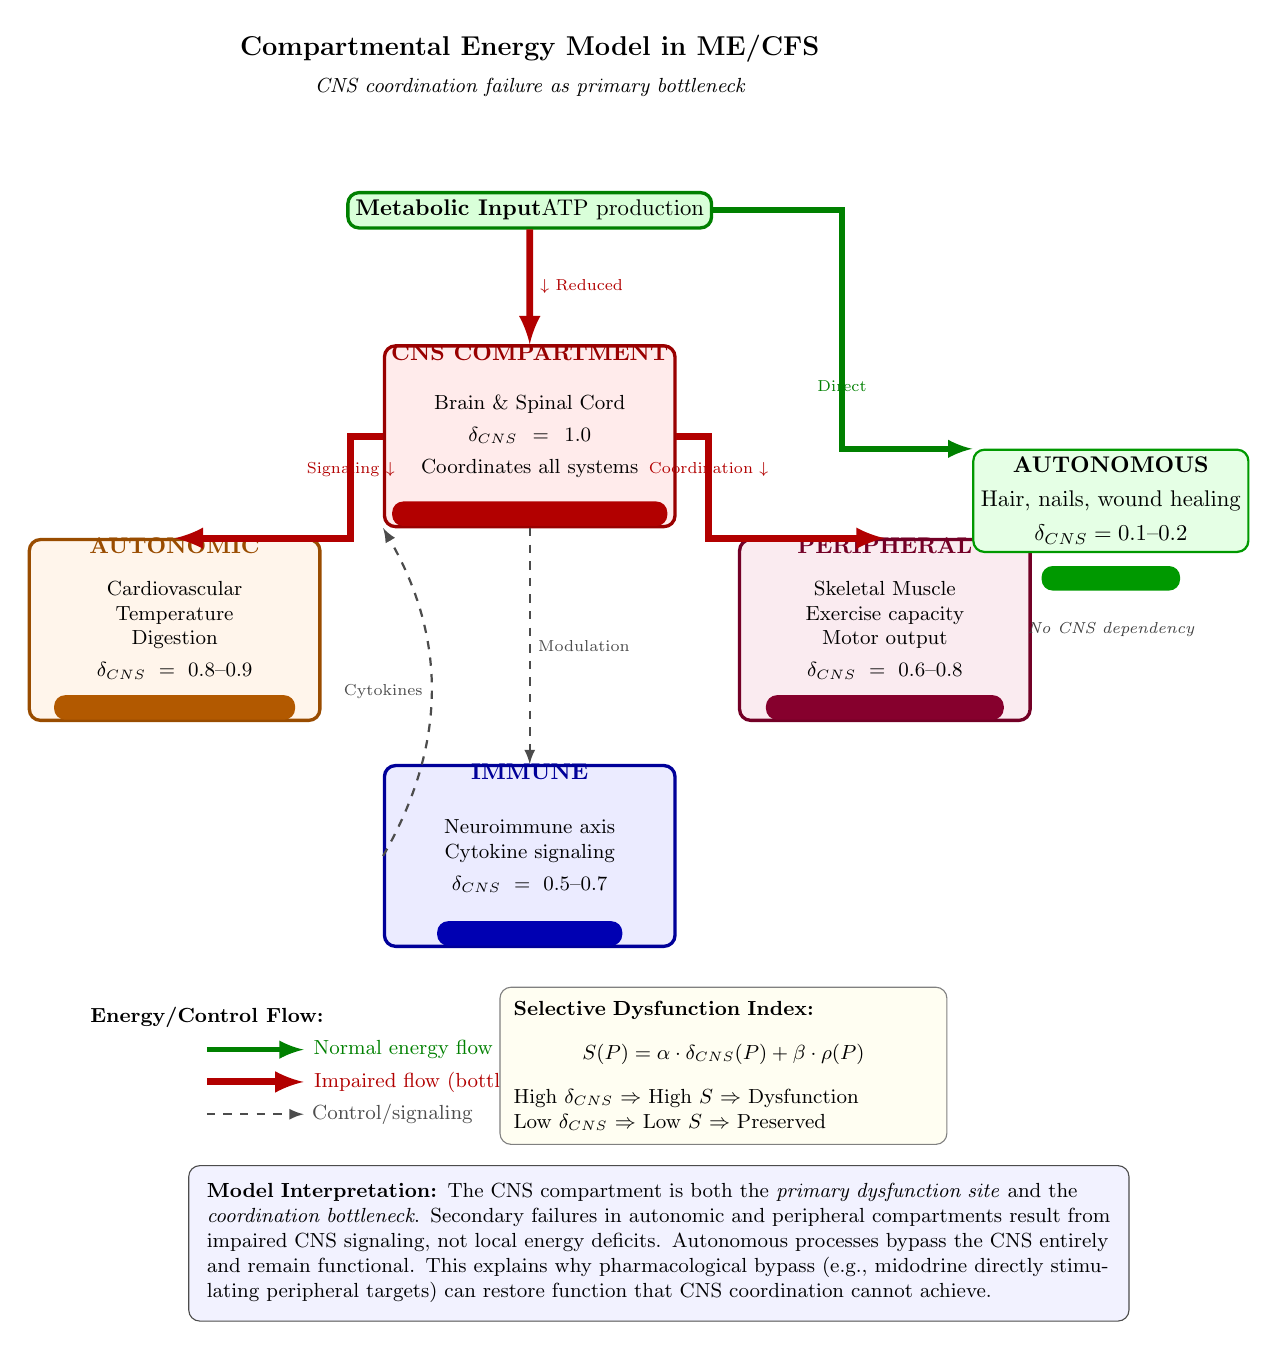
\begin{tikzpicture}[
    scale=0.82, every node/.style={scale=0.82},
    % Compartment styles
    compartment/.style={draw=black!70, very thick, rounded corners, minimum width=4.5cm, minimum height=2.8cm, align=center},
    cns-comp/.style={compartment, draw=red!60!black, fill=red!8},
    auto-comp/.style={compartment, draw=orange!60!black, fill=orange!8},
    periph-comp/.style={compartment, draw=purple!60!black, fill=purple!8},
    immune-comp/.style={compartment, draw=blue!60!black, fill=blue!8},
    preserved-comp/.style={draw=green!60!black, fill=green!10, thick, rounded corners, minimum width=3cm, minimum height=1.5cm, align=center},
    % Arrow styles
    energy-flow/.style={-latex, very thick, line width=2pt},
    control/.style={-latex, thick, dashed, gray!60!black},
    impaired/.style={-latex, ultra thick, red!70!black, line width=2.5pt},
    % Status indicators
    status/.style={font=\scriptsize\bfseries, rounded corners, inner sep=3pt},
]

% Title
\node[font=\large\bfseries] at (0, 9) {Compartmental Energy Model in ME/CFS};
\node[font=\small\itshape] at (0, 8.4) {CNS coordination failure as primary bottleneck};

% === ENERGY INPUT (top) ===
\node[draw=green!50!black, fill=green!15, very thick, rounded corners, minimum width=3cm] (input) at (0, 6.5) {\textbf{Metabolic Input}\\ATP production};

% === CNS COMPARTMENT (center, primary) ===
\node[cns-comp] (cns) at (0, 3) {};
\node[font=\bfseries, red!60!black] at (0, 4.3) {CNS COMPARTMENT};
\node[font=\small, text width=4cm, align=center] at (0, 3) {
    Brain \& Spinal Cord\\[3pt]
    $\delta_{CNS} = 1.0$\\[3pt]
    Coordinates all systems
};
\node[status, fill=red!20, red!70!black] at (0, 1.8) {PRIMARY DYSFUNCTION};

% Energy to CNS (impaired)
\draw[impaired] (input) -- (cns) node[midway, right, font=\scriptsize] {$\downarrow$ Reduced};

% === AUTONOMIC COMPARTMENT (left) ===
\node[auto-comp] (auto) at (-5.5, 0) {};
\node[font=\bfseries, orange!60!black] at (-5.5, 1.3) {AUTONOMIC};
\node[font=\small, text width=4cm, align=center] at (-5.5, 0) {
    Cardiovascular\\
    Temperature\\
    Digestion\\[3pt]
    $\delta_{CNS} = 0.8$--$0.9$
};
\node[status, fill=orange!20, orange!70!black] at (-5.5, -1.2) {SECONDARY FAILURE};

% CNS control to Autonomic (impaired)
\draw[impaired] (cns.west) -- ++(-0.5,0) |- (auto.north) node[pos=0.25, above, font=\scriptsize] {Signaling $\downarrow$};

% === PERIPHERAL COMPARTMENT (right) ===
\node[periph-comp] (periph) at (5.5, 0) {};
\node[font=\bfseries, purple!60!black] at (5.5, 1.3) {PERIPHERAL};
\node[font=\small, text width=4cm, align=center] at (5.5, 0) {
    Skeletal Muscle\\
    Exercise capacity\\
    Motor output\\[3pt]
    $\delta_{CNS} = 0.6$--$0.8$
};
\node[status, fill=purple!20, purple!70!black] at (5.5, -1.2) {COORDINATION LOSS};

% CNS control to Peripheral (impaired)
\draw[impaired] (cns.east) -- ++(0.5,0) |- (periph.north) node[pos=0.25, above, font=\scriptsize] {Coordination $\downarrow$};

% === IMMUNE COMPARTMENT (bottom) ===
\node[immune-comp] (immune) at (0, -3.5) {};
\node[font=\bfseries, blue!60!black] at (0, -2.2) {IMMUNE};
\node[font=\small, text width=4cm, align=center] at (0, -3.5) {
    Neuroimmune axis\\
    Cytokine signaling\\[3pt]
    $\delta_{CNS} = 0.5$--$0.7$
};
\node[status, fill=blue!20, blue!70!black] at (0, -4.7) {DYSREGULATED};

% CNS control to Immune
\draw[control] (cns.south) -- (immune.north) node[midway, right, font=\scriptsize] {Modulation};

% Feedback from immune to CNS
\draw[control, bend right=30] (immune.west) to node[midway, left, font=\scriptsize] {Cytokines} (cns.south west);

% === PRESERVED AUTONOMOUS PROCESSES (far right) ===
\begin{scope}[xshift=9cm, yshift=2cm]
    \node[preserved-comp] (pres) at (0, 0) {
        \textbf{AUTONOMOUS}\\[3pt]
        Hair, nails, wound healing\\[3pt]
        $\delta_{CNS} = 0.1$--$0.2$
    };
    \node[status, fill=green!20, green!60!black] at (0, -1.2) {PRESERVED};

    % Direct energy (bypasses CNS)
    \draw[energy-flow, green!50!black] (input.east) -- ++(2,0) |- (pres.north west) node[pos=0.4, above, font=\scriptsize] {Direct};

    % No CNS connection (explicit)
    \node[font=\scriptsize\itshape, gray!50!black] at (0, -2) {No CNS dependency};
\end{scope}

% === ENERGY FLOW LEGEND ===
\begin{scope}[yshift=-6.5cm, xshift=-5cm]
    \node[font=\small\bfseries] at (0, 0.5) {Energy/Control Flow:};
    \draw[energy-flow, green!50!black] (0, 0) -- (1.5, 0) node[right, font=\small] {Normal energy flow};
    \draw[impaired] (0, -0.5) -- (1.5, -0.5) node[right, font=\small] {Impaired flow (bottleneck)};
    \draw[control] (0, -1) -- (1.5, -1) node[right, font=\small] {Control/signaling};
\end{scope}

% === QUANTITATIVE MODEL ===
\begin{scope}[yshift=-6.5cm, xshift=3cm]
    \node[draw=black!50, fill=yellow!5, rounded corners, text width=6.5cm, align=left, font=\small, inner sep=6pt] at (0, -0.25) {
    \textbf{Selective Dysfunction Index:}
    \[
    S(P) = \alpha \cdot \delta_{CNS}(P) + \beta \cdot \rho(P)
    \]
    High $\delta_{CNS}$ $\Rightarrow$ High $S$ $\Rightarrow$ Dysfunction\\
    Low $\delta_{CNS}$ $\Rightarrow$ Low $S$ $\Rightarrow$ Preserved
    };
\end{scope}

% === KEY INSIGHT ===
\node[draw=black!70, fill=blue!5, rounded corners, text width=14cm, align=left, font=\small, inner sep=8pt] at (2, -9.5) {
\textbf{Model Interpretation:} The CNS compartment is both the \emph{primary dysfunction site} and the \emph{coordination bottleneck}. Secondary failures in autonomic and peripheral compartments result from impaired CNS signaling, not local energy deficits. Autonomous processes bypass the CNS entirely and remain functional. This explains why pharmacological bypass (e.g., midodrine directly stimulating peripheral targets) can restore function that CNS coordination cannot achieve.
};

\end{tikzpicture}
\caption{Four-compartment energy model showing CNS as the coordination bottleneck in ME/CFS. Compartments are classified by CNS-dependency index ($\delta_{CNS}$). Secondary dysfunction in autonomic and peripheral compartments results from impaired CNS coordination, while autonomous processes with $\delta_{CNS} < 0.2$ remain preserved.}
\label{fig:compartmental-energy-model}
\end{figure}
